\section{Q-Learning}

\begin{frame}
	\frametitle{}
	
	\Huge
	
	\vspace{0.5cm}
	
	\begin{center}
		\textbf{Q-Learning}
	\end{center}
\end{frame}

\begin{frame}
	\frametitle{Markov Decision Process (recap)}
	
	\large
	
	A finite discrete-time MDP is a tuple $ (\mathbf{S},\mathbf{A},\mathbf{P}_{sa}
	\mathbf{R},\gamma) $ where:
	
	\begin{itemize}
		\item $ \mathbf{S} $ is a finite set of N states
		\vspace{0.1cm}
		\item  $ \mathbf{A} = \{ a_1, a_2, \ldots, a_k \} $ is a set of $ k $ actions
		\vspace{0.1cm}
		\item $ \mathbf{P}_{sa}(\cdot) $ are the state transition probabilities upon taking
			  action $ a $ in a state $ s $
		\vspace{0.1cm}
		\item $ \mathbf{R} : \mathbf{S} \times \mathbf{A}  \mapsto \mathds{R} $ is the
			  reinforcement function, bounded in absolute value by $ R_{max} $
		\vspace{0.1cm}
		\item $ \gamma \in [0,1] $ is the discount factor
	\end{itemize}
\end{frame}

\begin{frame}
	\frametitle{State Representation (recap)}
	
	Typically a uniform grid $ N \times M $.
	
	\begin{table}[h]
		\begin{tabular}{|c|c|c|c|c|c|c|c|c|c|c|c|c|c|c|c|c|c|c|}
			\hline
			$ S_{11} $ & \multicolumn{17}{c|}{$ \;\;\;\;\;\;\;\;\;\;\;\;\;\;\;\;\;\;\;\;\;\;\;\;\;\;\;\; \ldots \;\;\;\;\;\;\;\;\;\;\;\;\;\;\;\;\;\;\;\;\;\;\;\;\;\;\;\; $} & $ S_{1M} $ \\ \hline
			\multirow{8}{*}{} & \multicolumn{17}{c|} {\multirow{8}{*}{}} & \multirow{8}{*}{} \\
			& \multicolumn{17}{c|}{} & \\
			& \multicolumn{17}{c|}{} & \\
			$ \vdots $ & \multicolumn{17}{c|}{$ \;\;\;\;\;\;\;\;\;\;\;\;\;\;\;\;\;\;\;\;\;\;\;\;\;\;\;\; \ddots \;\;\;\;\;\;\;\;\;\;\;\;\;\;\;\;\;\;\;\;\;\;\;\;\;\;\;\; $} & $ \vdots $ \\
			& \multicolumn{17}{c|}{} & \\
			& \multicolumn{17}{c|}{} & \\
			& \multicolumn{17}{c|}{} & \\ \hline
			$ S_{N1} $ & \multicolumn{17}{c|}{$ \;\;\;\;\;\;\;\;\;\;\;\;\;\;\;\;\;\;\;\;\;\;\;\;\;\;\;\; \ldots \;\;\;\;\;\;\;\;\;\;\;\;\;\;\;\;\;\;\;\;\;\;\;\;\;\;\;\; $} & $ S_{NM} $ \\ \hline
		\end{tabular}
	\end{table}
\end{frame}

\begin{frame}
	\frametitle{On-Policy/Off-Policy Learning (recap)}
	
	\Large
	
	\begin{itemize}
		\item \textbf{On-Policy Learning: } a learner learns the value of the optimal
			  policy independently of the agent's actions.
		\vspace{0.2cm}
		\item \textbf{Off-Policy Learning: } a learner learns the value of the policy being
			  carried out by the agent, including the exploration steps.
	\end{itemize}
\end{frame}

\begin{frame}
	\frametitle{Q-Learning (recap)}
	
	\Large
	
	\vspace{0.8cm}
	
	One of the most important breakthroughs in RL was the development of a Temporal
	Difference control algorithm known as \textbf{Q-learning} (Watkins, 1989).
	
	\vspace{0.5cm}
	
	Its simplest form, \emph{one-step Q-learning}, is defined by:
	
	\vspace{-0.4cm}
	
	\begin{equation*}
		Q(s_t,a_t) \leftarrow Q(s_t,a_t) + \alpha \Big [ r_{t + 1} + \gamma \max_a Q(s_{t + 1},a) - Q(s_t,a_t) \Big ]
	\end{equation*}
\end{frame}

\begin{frame}
	\frametitle{Q-Learning (recap)}
	\framesubtitle{Pseudo-code}
	
	\begin{algorithm}[H]
		\caption{Q-Learning}
		\BlankLine
		Initialize $ Q(s,a) $ arbitrarily
		\BlankLine
		Repeat (for each episode):\\
		{
			\hspace{0.7cm}
			Initialize $ s $ \\
			\hspace{0.7cm}
			Repeat (for each step of episode): \\
			{
				\hspace{1.4cm}
				Choose $ a $ from $ s $ using policy derived from $ Q $
				(e.g., $ \epsilon $-greedy) \\
				\hspace{1.4cm}
				Take action $ a $, observe $ r $, $ s^\prime $ \\
				\hspace{1.4cm}
				$ Q(s,a) \leftarrow Q(s,a) + \alpha \Big [ r + \gamma \max_{a^\prime}
				  Q(s^\prime,a^\prime) - Q(s,a) \Big ] $ \\
				\hspace{1.4cm}
				$ s \leftarrow s^\prime $ \\
			}
			\hspace{0.7cm}
			until $ s $ is terminal
		}
	\end{algorithm}
\end{frame}

\begin{frame}
	\frametitle{Exercise 1}
	
	\Large
	
	\begin{center}
		Is Q-Learning considered an \emph{on-policy} or \emph{off-policy} control method?
		Why?
	\end{center}
\end{frame}

\begin{frame}
	\frametitle{Q-Learning: Example}
	
	\vspace{0.4cm}
	
	\Large
	
	Consider the following grid world:
	
	\vspace{-0.2cm}
	
	\begin{figure}[!t]
		\centering
		\vspace{0.2cm}
		\begin{tikzpicture}[map/.style={draw=white,ultra thick,inner sep=0pt}]
			\node at (0,0) [map]
			{
				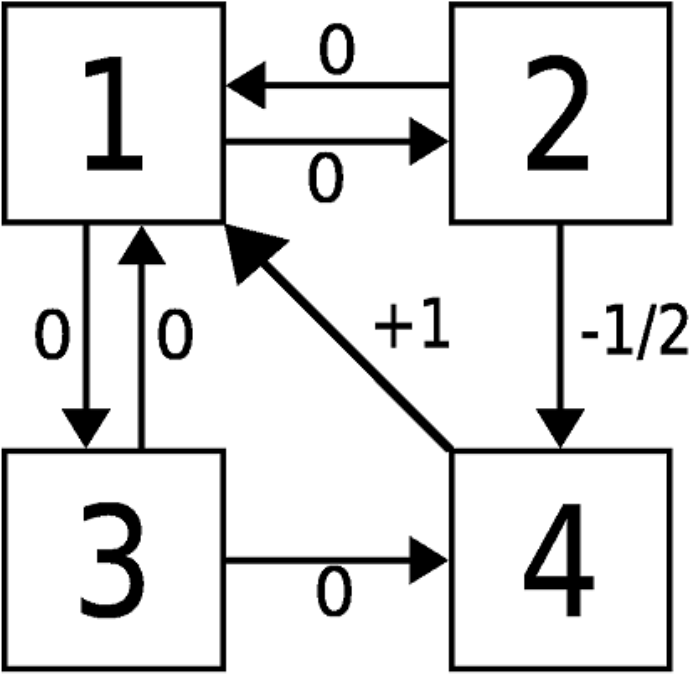
\includegraphics[width=0.5\linewidth]{Figures/GridWorld}
			};
		\end{tikzpicture}
	\end{figure}
\end{frame}

\begin{frame}
	\frametitle{Q-Learning: Example - cont'd}
	
	\Large
	
	An agent can move in the grid world to the \emph{left}, to the \emph{right}, \emph{up}
	and \emph{down}.
	
	\vspace{0.4cm}
	
	If it tries to \emph{move out} of the grid world, it will be \emph{punished} by a
	reward of $ -1 $.
	
	\vspace{0.4cm}
	
	\emph{Whatever} action the agent chose in state $ s_4 $, it will be automatically
	transferred to the state $ s_1 $ and will be \emph{granted} a reward of $ 1 $. \\
\end{frame}

\begin{frame}
	\frametitle{Q-Learning: Example - cont'd}
	
	\Large
	
	\begin{enumerate}
		\item Write down the MDP for this grid problem
		\item Apply Q-Learning algorithm assuming that the first agent's movements happened
			  to be: right, down, up, left, down, right, right. Let the discount factor be
			  $ 0.9 $, the starting state $ s_1 $ and $ \alpha = 0.1 $.
	\end{enumerate}
\end{frame}

\begin{frame}[<+->]
	\frametitle{Q-Learning: Example Solution}
	
	\vspace{0.4cm}
	
	\begin{enumerate}
		\item The corresponding MDP is deterministic and has the following form:
			  
			  \begin{itemize}
				  \item $ S = \{ s_1, s_2, s_3, s_4 \} $ - set of states
				  \vspace{0.15cm}
				  \item $ A = \{ LEFT, UP, RIGHT, DOWN \} $ - set of actions
				  \vspace{0.15cm}
				  \item $ \gamma = 0.9, \alpha = 0.1 $
				  \vspace{0.15cm}
				  \item State transition function:
						
						\begin{table}[!h]
							\scriptsize
							\begin{tabular}{c|c|c|c|c|}
								\cline{2-5}
								& \textbf{LEFT} & \textbf{UP} & \textbf{RIGHT} &
								\textbf{DOWN} \\ \hline
								\multicolumn{1}{|c|}{$ \mathbf{s_1} $} & $ s_1 $ & $ s_1 $
								& $ s_2 $ & $ s_3 $ \\ \hline
								\multicolumn{1}{|c|}{$ \mathbf{s_2} $} & $ s_1 $ & $ s_2 $
								& $ s_2 $ & $ s_4 $ \\ \hline
								\multicolumn{1}{|c|}{$ \mathbf{s_3} $} & $ s_3 $ & $ s_1 $    
								& $ s_4 $ & $ s_3 $ \\ \hline
								\multicolumn{1}{|c|}{$ \mathbf{s_4} $} & $ s_1 $ & $ s_1 $    
								& $ s_1 $ & $ s_1 $ \\ \hline
							\end{tabular}
						\end{table}
				  \vspace{0.15cm}
				  \item Reward function:
						
						\begin{table}[!h]
							\scriptsize
							\begin{tabular}{c|c|c|c|c|}
								\cline{2-5}
								& \textbf{LEFT} & \textbf{UP} & \textbf{RIGHT} &
								\textbf{DOWN} \\ \hline
								\multicolumn{1}{|c|}{$ \mathbf{s_1} $} & $ -1 $ & $ -1 $
								& $ 0 $ & $ 0 $ \\ \hline
								\multicolumn{1}{|c|}{$ \mathbf{s_2} $} & $ 0 $ & $ -1 $
								& $ -1 $ & $ -0.5 $ \\ \hline
								\multicolumn{1}{|c|}{$ \mathbf{s_3} $} & $ -1 $ & $ 0 $    
								& $ 0 $ & $ -1 $ \\ \hline
								\multicolumn{1}{|c|}{$ \mathbf{s_4} $} & $ 1 $ & $ 1 $    
								& $ 1 $ & $ 1 $ \\ \hline
							\end{tabular}
						\end{table}
			  \end{itemize}
	\end{enumerate}
\end{frame}

\begin{frame}[<+->]
	\frametitle{Q-Learning: Example Solution}
	
	\vspace{0.4cm}
	
	\begin{enumerate}
		\setcounter{enumi}{1}
		\item First, we initialize $ Q $-table with arbitrarily numbers (let it be zeros):
			  
			  \begin{table}[!h]
				  \begin{tabular}{c|c|c|c|c|}
					  \cline{2-5}
					  & \textbf{LEFT} & \textbf{UP} & \textbf{RIGHT} &
					  \textbf{DOWN} \\ \hline
					  \multicolumn{1}{|c|}{$ \mathbf{s_1} $} & $ 0 $ & $ 0 $
					  & $ 0 $ & $ 0 $ \\ \hline
					  \multicolumn{1}{|c|}{$ \mathbf{s_2} $} & $ 0 $ & $ 0 $
					  & $ 0 $ & $ 0 $ \\ \hline
					  \multicolumn{1}{|c|}{$ \mathbf{s_3} $} & $ 0 $ & $ 0 $    
					  & $ 0 $ & $ 0 $ \\ \hline
					  \multicolumn{1}{|c|}{$ \mathbf{s_4} $} & $ 0 $ & $ 0 $    
					  & $ 0 $ & $ 0 $ \\ \hline
				  \end{tabular}
			  \end{table}
			  
			  \vspace{0.4cm}
			  
			  The initial state (see conditions of the exercise) is $ s_1 $
	\end{enumerate}
\end{frame}

\begin{frame}[<+->]
	\frametitle{Q-Learning: Example Solution}
	\framesubtitle{Iteration 1}
	
	\vspace{0.5cm}
	
	\textbf{\underline{Q-Learning run (step 1):}}
	
	\begin{itemize}
		\item With probability $ 1 - \alpha $ = 0.9, we have to choose action $ a $ that
			  has maximal estimated action value \textcolor{red}{$ Q(s_1,a) $}, but with
			  probability $ \alpha = 0.1 $ we, instead, select a random action
		\item Since the $ Q $-table has all zeros, the first action is chosen completely
			  randomly. According to the condition of the exercise the first agent's
			  movements happened to be: right, down, up, left, down, right, right:
			  
			  \begin{center}
				  \textcolor{red}{$ a \leftarrow RIGHT $}
			  \end{center}
		\item We take action $ a $, observe the reward $ r = 0 $ and new state $
			  s^\prime = s_2 $
		\item \textcolor{red}{$ Q(s_1,R) $} $ \leftarrow Q(s_1,R) + \alpha \Big [ r + \gamma \max_{a^\prime} Q(s_2,a^\prime) - Q(s_1,R) \Big ] = 0 + 0.1 \cdot [ 0 + 0.9 \cdot 0 - 0 ] = $ \textcolor{red}{$ 0 $}
		\item \textcolor{red}{$ s \leftarrow s_2 $}
	\end{itemize}
\end{frame}

\begin{frame}
	\frametitle{Q-Learning: Example Solution}
	\framesubtitle{Iteration 1}
	
	\Large
	
	$ Q $-table after iteration 1 is the following:
	
	\begin{table}[!h]
		\begin{tabular}{c|c|c|c|c|}
			\cline{2-5}
			& \textbf{LEFT} & \textbf{UP} & \textbf{RIGHT} & \textbf{DOWN} \\ \hline
			\multicolumn{1}{|c|}{$ \mathbf{s_1} $} & $ 0 $ & $ 0 $ & $ 0 $ & $ 0 $\\ \hline
			\multicolumn{1}{|c|}{$ \mathbf{s_2} $} & $ 0 $ & $ 0 $ & $ 0 $ & $ 0 $\\ \hline
			\multicolumn{1}{|c|}{$ \mathbf{s_3} $} & $ 0 $ & $ 0 $ & $ 0 $ & $ 0 $\\ \hline
			\multicolumn{1}{|c|}{$ \mathbf{s_4} $} & $ 0 $ & $ 0 $ & $ 0 $ & $ 0 $\\ \hline
		\end{tabular}
	\end{table}
\end{frame}

\begin{frame}[<+->]
	\frametitle{Q-Learning: Example Solution}
	\framesubtitle{Iteration 2}
	
	\vspace{0.5cm}
	
	\textbf{\underline{Q-Learning run (step 2):}}
	
	\begin{itemize}
		\item With probability $ 1 - \alpha $ = 0.9, we have to choose action $ a $ that
			  has maximal estimated action value \textcolor{red}{$ Q(s_2,a) $}, but with
			  probability $ \alpha = 0.1 $ we, instead, select a random action:
			  
			  \begin{center}
				  \textcolor{red}{$ a \leftarrow DOWN $}
			  \end{center}
		\item We take action $ a $, observe the reward $ r = -0.5 $ and new state $
			  s^\prime = s_4 $
		\item \textcolor{red}{$ Q(s_2,D) $} $ \leftarrow Q(s_2,D) + \alpha \Big [ r + \gamma \max_{a^\prime} Q(s_4,a^\prime) - Q(s_2,D) \Big ] = 0 + 0.1 \cdot [ -0.5 + 0.9 \cdot 0 - 0 ] = $ \textcolor{red}{$ -0.05 $}
		\item \textcolor{red}{$ s \leftarrow s_4 $}
	\end{itemize}
\end{frame}

\begin{frame}
	\frametitle{Q-Learning: Example Solution}
	\framesubtitle{Iteration 2}
	
	\Large
	
	$ Q $-table after iteration 2 is the following:
	
	\begin{table}[!h]
		\begin{tabular}{c|c|c|c|c|}
			\cline{2-5}
			& \textbf{LEFT} & \textbf{UP} & \textbf{RIGHT} & \textbf{DOWN} \\ \hline
			\multicolumn{1}{|c|}{$ \mathbf{s_1} $} & $ 0 $ & $ 0 $ & $ 0 $ & $ 0 $\\ \hline
			\multicolumn{1}{|c|}{$ \mathbf{s_2} $} & $ 0 $ & $ 0 $ & $ 0 $ & $ -0.05 $\\ \hline
			\multicolumn{1}{|c|}{$ \mathbf{s_3} $} & $ 0 $ & $ 0 $ & $ 0 $ & $ 0 $\\ \hline
			\multicolumn{1}{|c|}{$ \mathbf{s_4} $} & $ 0 $ & $ 0 $ & $ 0 $ & $ 0 $\\ \hline
		\end{tabular}
	\end{table}
\end{frame}

\begin{frame}[<+->]
	\frametitle{Q-Learning: Example Solution}
	\framesubtitle{Iteration 3}
	
	\vspace{0.5cm}
	
	\textbf{\underline{Q-Learning run (step 3):}}
	
	\begin{itemize}
		\item With probability $ 1 - \alpha $ = 0.9, we have to choose action $ a $ that
			  has maximal estimated action value \textcolor{red}{$ Q(s_4,a) $}, but with
			  probability $ \alpha = 0.1 $ we, instead, select a random action:
			  
			  \begin{center}
				  \textcolor{red}{$ a \leftarrow UP $}
			  \end{center}
		\item We take action $ a $, observe the reward $ r = 1 $ and new state $
			  s^\prime = s_1 $
		\item \textcolor{red}{$ Q(s_4,U) $} $ \leftarrow Q(s_4,U) + \alpha \Big [ r + \gamma \max_{a^\prime} Q(s_1,a^\prime) - Q(s_4,U) \Big ] = 0 + 0.1 \cdot [ 1 + 0.9 \cdot 0 - 0 ] = $ \textcolor{red}{$ 0.1 $}
		\item \textcolor{red}{$ s \leftarrow s_1 $}
	\end{itemize}
\end{frame}

\begin{frame}
	\frametitle{Q-Learning: Example Solution}
	\framesubtitle{Iteration 3}
	
	\Large
	
	$ Q $-table after iteration 3 is the following:
	
	\begin{table}[!h]
		\begin{tabular}{c|c|c|c|c|}
			\cline{2-5}
			& \textbf{LEFT} & \textbf{UP} & \textbf{RIGHT} & \textbf{DOWN} \\ \hline
			\multicolumn{1}{|c|}{$ \mathbf{s_1} $} & $ 0 $ & $ 0 $ & $ 0 $ & $ 0 $\\ \hline
			\multicolumn{1}{|c|}{$ \mathbf{s_2} $} & $ 0 $ & $ 0 $ & $ 0 $ & $ -0.05 $\\ \hline
			\multicolumn{1}{|c|}{$ \mathbf{s_3} $} & $ 0 $ & $ 0 $ & $ 0 $ & $ 0 $\\ \hline
			\multicolumn{1}{|c|}{$ \mathbf{s_4} $} & $ 0 $ & $ 0.1 $ & $ 0 $ & $ 0 $\\ \hline
		\end{tabular}
	\end{table}
\end{frame}

\begin{frame}[<+->]
	\frametitle{Q-Learning: Example Solution}
	\framesubtitle{Iteration 4}
	
	\vspace{0.5cm}
	
	\textbf{\underline{Q-Learning run (step 4):}}
	
	\begin{itemize}
		\item With probability $ 1 - \alpha $ = 0.9, we have to choose action $ a $ that
			  has maximal estimated action value \textcolor{red}{$ Q(s_1,a) $}, but with
			  probability $ \alpha = 0.1 $ we, instead, select a random action:
			  
			  \begin{center}
				  \textcolor{red}{$ a \leftarrow LEFT $}
			  \end{center}
		\item We take action $ a $, observe the reward $ r = -1 $ and new state $
			  s^\prime = s_1 $
		\item \textcolor{red}{$ Q(s_1,L) $} $ \leftarrow Q(s_1,L) + \alpha \Big [ r + \gamma \max_{a^\prime} Q(s_1,a^\prime) - Q(s_1,L) \Big ] = 0 + 0.1 \cdot [ -1 + 0.9 \cdot 0 - 0 ] = $ \textcolor{red}{$ -0.1 $}
		\item \textcolor{red}{$ s \leftarrow s_1 $}
	\end{itemize}
\end{frame}

\begin{frame}
	\frametitle{Q-Learning: Example Solution}
	\framesubtitle{Iteration 4}
	
	\Large
	
	$ Q $-table after iteration 4 is the following:
	
	\begin{table}[!h]
		\begin{tabular}{c|c|c|c|c|}
			\cline{2-5}
			& \textbf{LEFT} & \textbf{UP} & \textbf{RIGHT} & \textbf{DOWN} \\ \hline
			\multicolumn{1}{|c|}{$ \mathbf{s_1} $} & $ -0.1 $ & $ 0 $ & $ 0 $ & $ 0 $\\ \hline
			\multicolumn{1}{|c|}{$ \mathbf{s_2} $} & $ 0 $ & $ 0 $ & $ 0 $ & $ -0.05 $\\ \hline
			\multicolumn{1}{|c|}{$ \mathbf{s_3} $} & $ 0 $ & $ 0 $ & $ 0 $ & $ 0 $\\ \hline
			\multicolumn{1}{|c|}{$ \mathbf{s_4} $} & $ 0 $ & $ 0.1 $ & $ 0 $ & $ 0 $\\ \hline
		\end{tabular}
	\end{table}
\end{frame}

\begin{frame}[<+->]
	\frametitle{Q-Learning: Example Solution}
	\framesubtitle{Iteration 5}
	
	\vspace{0.5cm}
	
	\textbf{\underline{Q-Learning run (step 5):}}
	
	\begin{itemize}
		\item With probability $ 1 - \alpha $ = 0.9, we have to choose action $ a $ that
			  has maximal estimated action value \textcolor{red}{$ Q(s_1,a) $}, but with
			  probability $ \alpha = 0.1 $ we, instead, select a random action:
			  
			  \begin{center}
				  \textcolor{red}{$ a \leftarrow DOWN $}
			  \end{center}
		\item We take action $ a $, observe the reward $ r = 0 $ and new state $
			  s^\prime = s_3 $
		\item \textcolor{red}{$ Q(s_1,D) $} $ \leftarrow Q(s_1,D) + \alpha \Big [ r + \gamma \max_{a^\prime} Q(s_3,a^\prime) - Q(s_1,D) \Big ] = 0 + 0.1 \cdot [ 0 + 0.9 \cdot 0 - 0 ] = $ \textcolor{red}{$ -0.1 $}
		\item \textcolor{red}{$ s \leftarrow s_3 $}
	\end{itemize}
\end{frame}

\begin{frame}
	\frametitle{Q-Learning: Example Solution}
	\framesubtitle{Iteration 5}
	
	\Large
	
	$ Q $-table after iteration 5 is the following:
	
	\begin{table}[!h]
		\begin{tabular}{c|c|c|c|c|}
			\cline{2-5}
			& \textbf{LEFT} & \textbf{UP} & \textbf{RIGHT} & \textbf{DOWN} \\ \hline
			\multicolumn{1}{|c|}{$ \mathbf{s_1} $} & $ -0.1 $ & $ 0 $ & $ 0 $ & $ 0 $\\ \hline
			\multicolumn{1}{|c|}{$ \mathbf{s_2} $} & $ 0 $ & $ 0 $ & $ 0 $ & $ -0.05 $\\ \hline
			\multicolumn{1}{|c|}{$ \mathbf{s_3} $} & $ 0 $ & $ 0 $ & $ 0 $ & $ 0 $\\ \hline
			\multicolumn{1}{|c|}{$ \mathbf{s_4} $} & $ 0 $ & $ 0.1 $ & $ 0 $ & $ 0 $\\ \hline
		\end{tabular}
	\end{table}
\end{frame}

\begin{frame}[<+->]
	\frametitle{Q-Learning: Example Solution}
	\framesubtitle{Iteration 6}
	
	\vspace{0.5cm}
	
	\textbf{\underline{Q-Learning run (step 6):}}
	
	\begin{itemize}
		\item With probability $ 1 - \alpha $ = 0.9, we have to choose action $ a $ that
			  has maximal estimated action value \textcolor{red}{$ Q(s_3,a) $}, but with
			  probability $ \alpha = 0.1 $ we, instead, select a random action:
			  
			  \begin{center}
				  \textcolor{red}{$ a \leftarrow RIGHT $}
			  \end{center}
		\item We take action $ a $, observe the reward $ r = 0 $ and new state $
			  s^\prime = s_3 $
		\item \textcolor{red}{$ Q(s_3,R) $} $ \leftarrow Q(s_3,R) + \alpha \Big [ r + \gamma \max_{a^\prime} Q(s_4,a^\prime) - Q(s_3,R) \Big ] = 0 + 0.1 \cdot [ 0 + 0.9 \cdot 0.1 - 0 ] = $ \textcolor{red}{$ 0.009 $}
		\item \textcolor{red}{$ s \leftarrow s_4 $}
	\end{itemize}
\end{frame}

\begin{frame}
	\frametitle{Q-Learning: Example Solution}
	\framesubtitle{Iteration 6}
	
	\Large
	
	$ Q $-table after iteration 6 is the following:
	
	\begin{table}[!h]
		\begin{tabular}{c|c|c|c|c|}
			\cline{2-5}
			& \textbf{LEFT} & \textbf{UP} & \textbf{RIGHT} & \textbf{DOWN} \\ \hline
			\multicolumn{1}{|c|}{$ \mathbf{s_1} $} & $ -0.1 $ & $ 0 $ & $ 0 $ & $ 0 $\\ \hline
			\multicolumn{1}{|c|}{$ \mathbf{s_2} $} & $ 0 $ & $ 0 $ & $ 0 $ & $ -0.05 $\\ \hline
			\multicolumn{1}{|c|}{$ \mathbf{s_3} $} & $ 0 $ & $ 0 $ & $ 0.009 $ & $ 0 $\\ \hline
			\multicolumn{1}{|c|}{$ \mathbf{s_4} $} & $ 0 $ & $ 0.1 $ & $ 0 $ & $ 0 $\\ \hline
		\end{tabular}
	\end{table}
\end{frame}

\begin{frame}[<+->]
	\frametitle{Q-Learning: Example Solution}
	\framesubtitle{Iteration 7}
	
	\vspace{0.5cm}
	
	\textbf{\underline{Q-Learning run (step 7):}}
	
	\begin{itemize}
		\item With probability $ 1 - \alpha $ = 0.9, we have to choose action $ a $ that
			  has maximal estimated action value \textcolor{red}{$ Q(s_4,a) $}, but with
			  probability $ \alpha = 0.1 $ we, instead, select a random action:
			  
			  \begin{center}
				  \textcolor{red}{$ a \leftarrow RIGHT $}
			  \end{center}
		\item We take action $ a $, observe the reward $ r = 1 $ and new state $
			  s^\prime = s_1 $
		\item \textcolor{red}{$ Q(s_4,R) $} $ \leftarrow Q(s_4,R) + \alpha \Big [ r + \gamma \max_{a^\prime} Q(s_1,a^\prime) - Q(s_4,R) \Big ] = 0 + 0.1 \cdot [ 1 + 0.9 \cdot 0 - 0 ] = $ \textcolor{red}{$ 0.1 $}
		\item \textcolor{red}{$ s \leftarrow s_1 $}
	\end{itemize}
\end{frame}

\begin{frame}
	\frametitle{Q-Learning: Example Solution}
	\framesubtitle{Iteration 7}
	
	\Large
	
	$ Q $-table after iteration 7 is the following:
	
	\begin{table}[!h]
		\begin{tabular}{c|c|c|c|c|}
			\cline{2-5}
			& \textbf{LEFT} & \textbf{UP} & \textbf{RIGHT} & \textbf{DOWN} \\ \hline
			\multicolumn{1}{|c|}{$ \mathbf{s_1} $} & $ -0.1 $ & $ 0 $ & $ 0 $ & $ 0 $\\ \hline
			\multicolumn{1}{|c|}{$ \mathbf{s_2} $} & $ 0 $ & $ 0 $ & $ 0 $ & $ -0.05 $\\ \hline
			\multicolumn{1}{|c|}{$ \mathbf{s_3} $} & $ 0 $ & $ 0 $ & $ 0.009 $ & $ 0 $\\ \hline
			\multicolumn{1}{|c|}{$ \mathbf{s_4} $} & $ 0 $ & $ 0.1 $ & $ 0.1 $ & $ 0 $\\ \hline
		\end{tabular}
	\end{table}
\end{frame}

\begin{frame}
	\frametitle{Q-Learning: Example Solution}
	\framesubtitle{Optimal policy trend}
	
	\large
	
	\vspace{0.2cm}
	
	It is clear that, $ Q $-table will take the form according to which one of the optimal
	policies will be \\
	
	\vspace{-0.2cm}
	
	\begin{center}
		\textcolor{red}{$ \pi^* : \pi^*(s_1) = DOWN, $} \\
		\textcolor{red}{$ \;\;\;\,\, \pi^*(s_2) = LEFT, $} \\
		\textcolor{red}{$ \;\;\;\;\;\,\, \pi^*(s_3) = RIGHT, $} \\
		\textcolor{red}{$ \;\;\;\,\,\,\, \pi^*(s_4) = DOWN $}
	\end{center}
	
	\vspace{-0.2cm}
	
	Other optimal policies will choose other actions $ (LEFT,RIGHT,UP) $ in state $ s_4 $.
	In state $ s_2 $ the agent has to choose action $ LEFT $ for even discounted reward on
	this way $ (0.9^3 \cdot 1) $ is greater than immediate reward $ -0.5 $ and then reward
	$ 1 $ discounted by $ \gamma = 0.9 $ \\
\end{frame}
